\chapter{Dokumentacja kodu}

\section{Użyte technologie}
Całość systemu została zaimplementowana w jęzku obiektowym \textbf{Java 8} przy użyciu narzędzi dostępnych w \textbf{Java EE} (ang. enterprise edition). Do automatyzacji budowania projektu w przypadku aplikajci webowej został wykorzystany \textbf{Maven}, natomiast jeśli chodzi o aplikacje webową był to \textbf{Gradle}. Framework w oparciu którego została napisana aplikacja mobilna jest \textbf{Retrofit}. Ułatwia on w znaczny sposób pracę z różnego typu HTML'owych API (ang. application programming interface), m.in REST API. Narzędzie w znaczny sposób ułatwiło nam mapowanie obiket na JSON'a oraz JSON'a na obiekty, jak również samo wysyłanie zapytań oraz odbieranie i interpretacja odpowiedzi serwera, pamietając o konieczności legitymacji się identyfikatorem sesji.

\paragraph{}
Jeśli chodzi o część systemu odpowiedzialną za aplikacje webową technologiami, które zostały wykorzystane są narzędzia z rodziny \textbf{Spring}. Program został zaprojektowany zgodnie z zasadami \textbf{GRASP},a podczas implementacji z zachowaniem tych zasadł pomógł nam \textbf{Spring Core}, ułatwiał on wykorzystanie wzorca \textbf{DI} (ang. Dependency Injection), co skutkowało zachowaniem niskiego sprzężenia oraz wyskokiej spójności klas. Znaczna większość obiektów, które były wstrzykiwane poprzez \textbf{DI} były przedstawicielami wzorca projektowego \textbf{Singleton}, co skutowało zmniejszeniem zapotrzebania na zasoby komputera naszego serwera. Singletonami są wszystkie klasy serwisowe, kontrolery oraz klasy konfiguracyjne. Poza klasami konfiguracyjnymi wszystkie klasy wstrzykiwane przy użyciu \textbf{Spring Core} były implementacjami interfesjów, co pozwoliło \textbf{Springowi} w bardzo lekki i łatwy sposób przy użyciu refleksji budowanie \textbf{Proxy} tych obiektów w trakcie uruchomienia aplikacji i załadowania kontekstu,a nie jak miałoby by to miejsce w przypadki gdyby obiekty wstrzykiwane rozszerzały klase (lub też nie rozserzały żadnej kalsy abstrakcyjnej) modyfikując kod bitowy, który został wcześniej skompilowany. W różnych częsiach projektu mieliśmy doczynienia z programowaniem aspektowym, które również było możliwe, dzięki \textbf{Spring Core} oraz wcześniej stworzonym \textbf{Proxy} do wstrzykiwanych klas. Framework, z którym najwięcej pracowaliśmy to \textbf{Spring MVC}. Jest to narzędzie, które umożliwia z jasny sposób budować aplikacje webowe w opraciu o wzorzec projektowy \textbf{MVC}. Dzięki niemu w łatwy sposób mogliśmy zbudować most łączący widok z modelem, czyli kontrolery. \textbf{Spring MVC} rownież ułatwił nam walidacje dancyh otrzymanych przez użytkowników poprzez pare na adnotacjach dostępnych w pakietach \textbf{javax.validation.api}. Wraz z \textbf{Spring MVC} wykorzystywany był \textbf{Jackson}, czyli biblioteka odpowiedzialana za mapowanie instancje klas na obiekty JSON, oraz w drugą stronę.

\paragraph{}
W zabezpieczaniu naszego systemu pomogły nam rownież \textbf{Spring Security} oraz \textbf{Spring Session}. Drugie z nich dawało nam większą kontrole nad sesjami i jej atrybutami (tak jak \textbf{CSRF tokeny} oraz blokowane kupony, które rownież wiązane były z sesją) jak również umożliwiało nam to przechowywanie identyfiaktorów sesji w bazie danych. Jeśli chodzi o \textbf{Spring Security} miał on wpływ na implementacja autoryzacji oraz uwierzytelniania w naszym serwisie. To narzędzie sprawdzało podczas otrzymania zapytania przez serwer, czy dany użytkownik legitymujący się identyfikatorem sesji ma odpowiednie uprawnienia do przeglądania danej podstrony jak również wywoływania metod zarówna w kontrolerze oraz w klasach serwisowych. Umożliwił w łatwy sposób również implementacje różnego typu handler'ów dla przypadków, gdy użytkownikowi nie udało się prawdiłowo zalogować/wylogować lub gdy właśnie probował przejść do strony, do której nie ma dostępu. Narzędzie to również automatycznie hashuje hasła podane przez użytkowników (po wcześniejszym zadeklarowaniu wybranego przez nas algorytmu haszującego), co jest znaczące jeśli chodzi o przechowywanie wrażliwych dla użytkoników danych.

\paragraph{}
Kolejnym narzędziem jest \textbf{Thymeleaf}, który został wykorzystanu do front-end'owej częsci projektu, czyli silnik umożliwiający tworzenie szablonów HTML, który jest w łatwy sposób jest integrowany ze \textbf{Spring MVC}.  Dzięki możliwości korzystania m.in. z pętl, branch'ów oraz fragmentów kod HTML'owy stworzony przy użyciu Thymeleafa jest spójny oraz czytelny, gdyż miejscami przypomina kod jakiegoś standardowego języka programowania. Podczas prac nad modelem zostały wykorzystane również : \textbf{JavaScript},\textbf{jQuery},\textbf{CSS}.

\paragraph{}
Przydatnym narzędziem okazały się również \textbf{Spring WebFlow} oraz \textbf{Spring Mail}, które oferują wysokopoziomowe interfejsy dla wielostopniowych formularzy (ang. wizards) oraz wysyłce maili o zadanych wcześniej wyglądach (szablonach HTML). Pełna integracja z kodem Javowym w narzędziu odpowiedzialnym za formularze jest nie do opisania, ponieważ dzięki temu w formularzach jesteśmy wstanie zastosować branche, pracować na wprowadzonych przez użytkownika danych, jak również je przetwarzać na każdym etapie wykonywania formualrza.

\paragraph{}
Narzędziami przez nas użytymi były rownież frameworki ORM (ang. Object-Relational Mapping), a chodzi tu o \textbf{Hibernate}. Poprzez właśnie to narzędzie następowała komunikacja z naszą bazą danych \textbf{MySQL}, czyli wprowadzanie,edycja oraz usuwanie danych. \textbf{Hibernate} odpowiedzialny był za mapowanie krotek bazodanowych na instacje klas Modelu oraz instacji klas modelu na zapytania SQL'owe. Wykorzystany został rownież do wygenerowania gotowej bazy danych, na której później pracowaliśmy.

\paragraph{}
Używamy również frameworka \texttt{caffeine}, który służy do cachowania. W naszym systemie są cachowane statystyki, które są elementem najbardziej obciążającym system. Cache ulega dezaktualizacji po 20 minutach i musi zostać wtedy odświeżony. Dodanie do systemu ankiety o danym \textit{id} powoduje również dezaktualizację cachu. Nie jest więc wykonywany niepotrzebny narzut pracy serwera, związany z dostarczaniem funkcjonalności statystyk w serwerze.

\section{Rejestracja}
\paragraph{}
Do implementacji mechanizmu rejestracji zostało wykorzystane narzędzie o nazwie \textbf{Spring WebFlow}, które jest wykorzystywane do wielostopniowego formularza (ang. wizard). W pliku XML-owym możemy odwoływac się do metod serwisowych, implementować na podstawie tego branch'e oraz decydowac na jakim etapie formularza jaka grupa walidacji będzie walidowana.
\begin{center}
\begin{lstlisting}[caption={Listing kodu odpowiedzialnego za rejestrację.},captionpos=b]
<?xml version="1.0" encoding="UTF-8"?>
<flow xmlns="http://www.springframework.org/schema/webflow"
      xmlns:xsi="http://www.w3.org/2001/XMLSchema-instance"
      xsi:schemaLocation="http://www.springframework.org/schema/webflow http://www.springframework.org/schema/webflow/spring-webflow-2.4.xsd">

    <var name="company" class="pwr.groupproject.vouchers.bean.form.NewUserCompanyForm"/>

    <view-state id="step1" view="/signup/signup1.html" model="company"
                validation-hints="'validationGroup1'" >
        <transition on="nextStep" to="step2">
            <evaluate expression="userCompanyServiceImpl.validateUserCompany(company,messageContext)" />
        </transition>
        <transition on="cancel" to="cancel" validate="false" bind="false" />
    </view-state>

    <view-state id="step2" view="/signup/signup2.html" model="company"
                validation-hints="'validationGroup2'">
        <transition on="nextStep" to="success">
            <evaluate expression="userCompanyServiceImpl.addUser(company)" />
        </transition>
        <transition on="cancel" to="cancel" validate="false" />
        <transition on="previousStep" to="step1" validate="false" />
    </view-state>

    <end-state id="success" view="externalRedirect:/?acc=1" />
    <end-state id="cancel" view="externalRedirect:/" />
</flow>
\end{lstlisting}
\end{center}
Dla pierwszego etapu rejestracji do modelu (który jest ten sam dla całego trwania procesu) dodawany jest pusty formularz, czyli obiekt w którym będziemy przechowywać wszystkie dane wprowadzone przez użytkownika. Następnie po zatwierdzeniu pierwszego etapu przez użytkownika , sprwadzamy czy wprowadzone dane są zgodne z wymogami przedstawionymi przez serwer (np. czy podany przez użytkownika adres e-mail nie znajduje się już w naszej bazie danych) poprzez $<evaluate expression="userCompanyServiceImpl.validateUserCompany(company,messageContext)" />$,  w której wywołujemy klase serwisową naszego systemu. W przypadku, gdy dane nie spełnią wymogów wyświetlamy odpowiednie komunikaty błędów, w których jasno informujemy klienta co należy zrobić, aby owe wymogi spełnić. W przypadku gdy dane zostaną zatwierdzone przez serwer przechodzimy do drugiego etapu formularza  $<view-state id="step2" ... </view-state>$. Tam użytkownik uzupełnia formularz kolejną serią danych (np. hasłem oraz jego powtórzeniem) po zatwierdzeniu których serwer poraz kolejny waliduje dane wejściowe, tym razem już cały formularz. W przypadku przejścia wszystkich wymogów walidacji zostaje wykonana instrukcja $<transition on="nextStep" to="success">...</transition>$, co skutkuje wywołanem funkcji serwisowej $addUser(obj: Company)$. Po pomyślnym dodaniu użytkownika do bazy danych proces trafia do linijki $25$ w powyższym listingu i zostaje przekierowany na strone startową, na której dzięki parametrowi ``acc'' wyświetli się odpowiedni komunikat informujący o konieczności aktywacji konta przed zalogowaniem się.


\section{Resetowanie hasła dla konta}
\paragraph{}
\begin{center}
\begin{lstlisting}[caption={Listing kodu obsługującego odzyskiwanie hasła.},captionpos=b]
@RequestMapping(value = "forgot_password", method = RequestMethod.GET)
public String forgottenPassword(Model model) {
	model.addAttribute("form", new ForgotPasswordForm());
	return "auth/forgot_password.html";
}

@RequestMapping(value = "forgot_password", method = RequestMethod.POST)
public String forgottenPassword(@ModelAttribute(name = "form") @Validated ForgotPasswordForm forgotPasswordForm, BindingResult bindingResult) {
	if (bindingResult.hasErrors())
		return "auth/forgot_password.html";

	UserCompany userCompany = userCompanyService.getUserByUserName(forgotPasswordForm.getUserName());
	if (userCompany == null) {
		bindingResult.rejectValue("userName", "email.dont.exist", messageSource.getMessage("message.wrong.email", null, LocaleContextHolder.getLocale()));
		return "auth/forgot_password.html";
	} else if (!userCompany.isEnabled()) {
		bindingResult.rejectValue("userName", "account.not.activated", messageSource.getMessage("messages.account.not.activated", null, LocaleContextHolder.getLocale()));
		return "auth/forgot_password.html";
	} else {
		PasswordResetToken passwordResetToken = tokenService.generateNewPasswordResetToken(userCompany);
		mailService.sendPasswordResetEmail(passwordResetToken.getToken(), userCompany.getUsername());
	}

	return "redirect:/?acc=5";
}
\end{lstlisting}
\end{center}
Metoda oznaczona adnotacją $@RequestMapping(value = "/reset_password", method = RequestMethod.GET)$ przygotowywuje pusty formularz który ma zawierać jedynie adres e-mail konta dla którego użytkownik chce zresetować hasło. W przypadku, gdy użytkownik poda adres e-mail, który faktycznie znajduje się w naszej bazie danych zostaje generowany jednorazowy token (co zostało przedstawione w listingu poniżej), który zostaje wysłany w mail'u na wcześniej wskazany adres e-mail.

\begin{center}
\begin{lstlisting}[caption={Listing kodu generującego token do odzyskiwania hasła.},captionpos=b]
@Override
public PasswordResetToken generateNewPasswordResetToken(UserCompany userCompany) {
	tokenDao.deleteUsersResetTokens(userCompany.getUsername());
	PasswordResetToken passwordResetToken = new PasswordResetToken();
	passwordResetToken.setUserCompany(userCompany);
	passwordResetToken.setToken(RandomString.make(TOKEN_LENGTH));
	tokenDao.addPasswordResetToken(passwordResetToken);
	return passwordResetToken;
}

@Override
public PasswordResetToken validatePasswordResetToken(String passwordResetToken) throws WrongTokenException {
	try {
		return tokenDao.getPasswordResetTokenByToken(passwordResetToken);
	} catch (NoResultException ex) {
		throw new WrongTokenException();
	}
}
\end{lstlisting}
\end{center}
Tylko i wyłącznie jeden token odpowiadający za resetowanie hasła może być pisany do konta, tak więc przed dodaniem nowego ``PasswordResetToken'' ewentualny obiekt, który mógł istnieć wcześniej jest kasowany.

\begin{center}
\begin{lstlisting}[caption={Listing kodu resetującego hasło.},captionpos=b]
@RequestMapping(value = "/reset_password", method = RequestMethod.GET)
public String resetPassword(@RequestParam("t") String token, Model model) {
	try {
		tokenService.validatePasswordResetToken(token);
		ResetPasswordForm form = new ResetPasswordForm();
		form.setResetPasswordToken(token);
		model.addAttribute("resetPasswordForm", form);
		model.addAttribute("tokenStatus", TokenStatus.OK);
	} catch (WrongTokenException ex) {
		model.addAttribute("tokenStatus", TokenStatus.WRONG);
	}
	return "token/reset_password.html";
}

@RequestMapping(value = "/reset_password", method = RequestMethod.POST)
public String resetPassword(@ModelAttribute @Validated ResetPasswordForm resetPasswordForm, BindingResult bindingResult, Model model) {
	if (bindingResult.hasErrors()) {
		try {
			tokenService.validatePasswordResetToken(resetPasswordForm.getResetPasswordToken());
			model.addAttribute("tokenStatus", TokenStatus.OK);
		} catch (WrongTokenException ex) {
			model.addAttribute("tokenStatus", TokenStatus.WRONG);
		}
		return "token/reset_password.html";
	}
	userCompanyService.changePassword(resetPasswordForm);
	return "token/reset_password_success.html";
}
\end{lstlisting}
\end{center}
Użytkownik klikający w link w mailu wysłanym przez nasz system przekazujemy w postaci parametru zapytani $GET$ wcześniej wygenerowany token. Po wcześniejszej walidacji tokenu użytkwonik jest przeniesiony do strony zawierający formularz, w którym podaje dwa razy to samo nowe hasło, którym od momentu potwierdzenia formularza będzie się posługiwał.


\section{Tworzenie ankiety}
\paragraph{}
Proces tworzenia ankiety zaczyna się w momencie wysłania żądania \texttt{GET} przez zalogowaną firmę pod adres \texttt{/surveys/add}. Po stronie klienta jest wczytywany panel do tworzenia ankiety pozwalający na bieżącą edycję ankiety w trakcie jej tworzenia. Panel pozwala na dowolne zmiany nazwy, opisu ankiety oraz kolejności pytań. Jest możliwe również usuwanie poszczególnych pytań z ankiety. Możliwy jest również podgląd ankiety w czasie rzeczywistym. Do pól odpowiadających za nazwę oraz opis ankiety są podłączone słuchacze zdarzeń, które po zmianie wartości wspomnianych pól wywołują \textit{callback}, wprowadzający zmiany w podglądzie ankiety. Pytania w czasie tworzenia ankiety są przechowywane w tablicy obiektów w języku \texttt{Javascript}. Każde dodane pytanie ma podmienianą treść przy użyciu wyrażenia regularnego, dzięki czemu od strony front-endu pytania zabezpieczane są przed próbą wstrzyknięcia złośliwego skryptu. Dla znaków \texttt{"}, \texttt{'}, \texttt{/}, \texttt{<} oraz \texttt{>} są stosowane sekwencje ucieczkowe.

\paragraph{}
Po nacisnięciu przycisku \texttt{Dodaj ankietę}, do serwera wysyłane jest żądanie \texttt{POST} zawierające w ciele \texttt{JSON}, który jest automatycznie mapowany na obiekt z języka \texttt{Java}, dzięki zastosowaniu parsera \texttt{Jackson}. Obiekt klasy \texttt{SurveyDto} jest walidowany pod kątem zawartości niedozwolonych znaków oraz braku pól pustych. Jeżeli walidacja się powiedzie, do klienta jest zwracana odpowiedź ze statusem \texttt{HttpServlet\linebreak Response.SC\_CREATED} i po stronie klienta następuje przekierowanie do panelu zarządzania ankietami. W przypadku, gdy walidacja się nie powiedzie, do klienta zwracana jest odpowiedź ze statusem \texttt{HttpServlet\linebreak Response.SC\_NOT\_ACCEPTABLE} i następuje powiadomienie o niepowodzeniu dodania ankiety.

\paragraph{}
Po udanej walidacji obiektu klasy \texttt{SurveyDto} wywoływana jest metoda \texttt{addSurvey} z serwisu \texttt{Company\-Survey\-Service}, która dodaje utworzoną ankietę do bazy danych. Przed dodaniem ankiety do bazy danych, na podstawie obiektu \texttt{SurveyDto} jest tworzony obiekt klasy \texttt{Survey}, który jest integralną częścią modelu aplikacji. Dzięki zastosowaniu obiektów klasy \texttt{SurveyDto} do komunikacji z klientem, możliwe jest oszczędność na przesyle danych, gdyż do komunikacji nie są wykorzystywane niepotrzebne z punktu widzenia klienta dane, używane jednakże w bazie. Szybsza komunikacja została uzyskana kosztem narzutu pracy serwera, którą trzeba przeznaczyć na mapowanie obiektu klasy \texttt{SurveyDto} na obiekt klasy \texttt{Survey}.

\paragraph{}
Zmapowany obiekt klasy \texttt{Survey} jest w kolejnym kroku zapisywany w bazie danych, przy użyciu frameworka \texttt{Hibernate}. Framework ten pozwala na relacyjno-obiektowe mapowanie, dzięki czemu zobowiązanie do zapisania obiektu do bazy danych może być przesunięte na ten framework. Więcej o działaniu frameworka w projekcie można przeczytać w rodziale trzecim.

\begin{figure}[h]
\centering
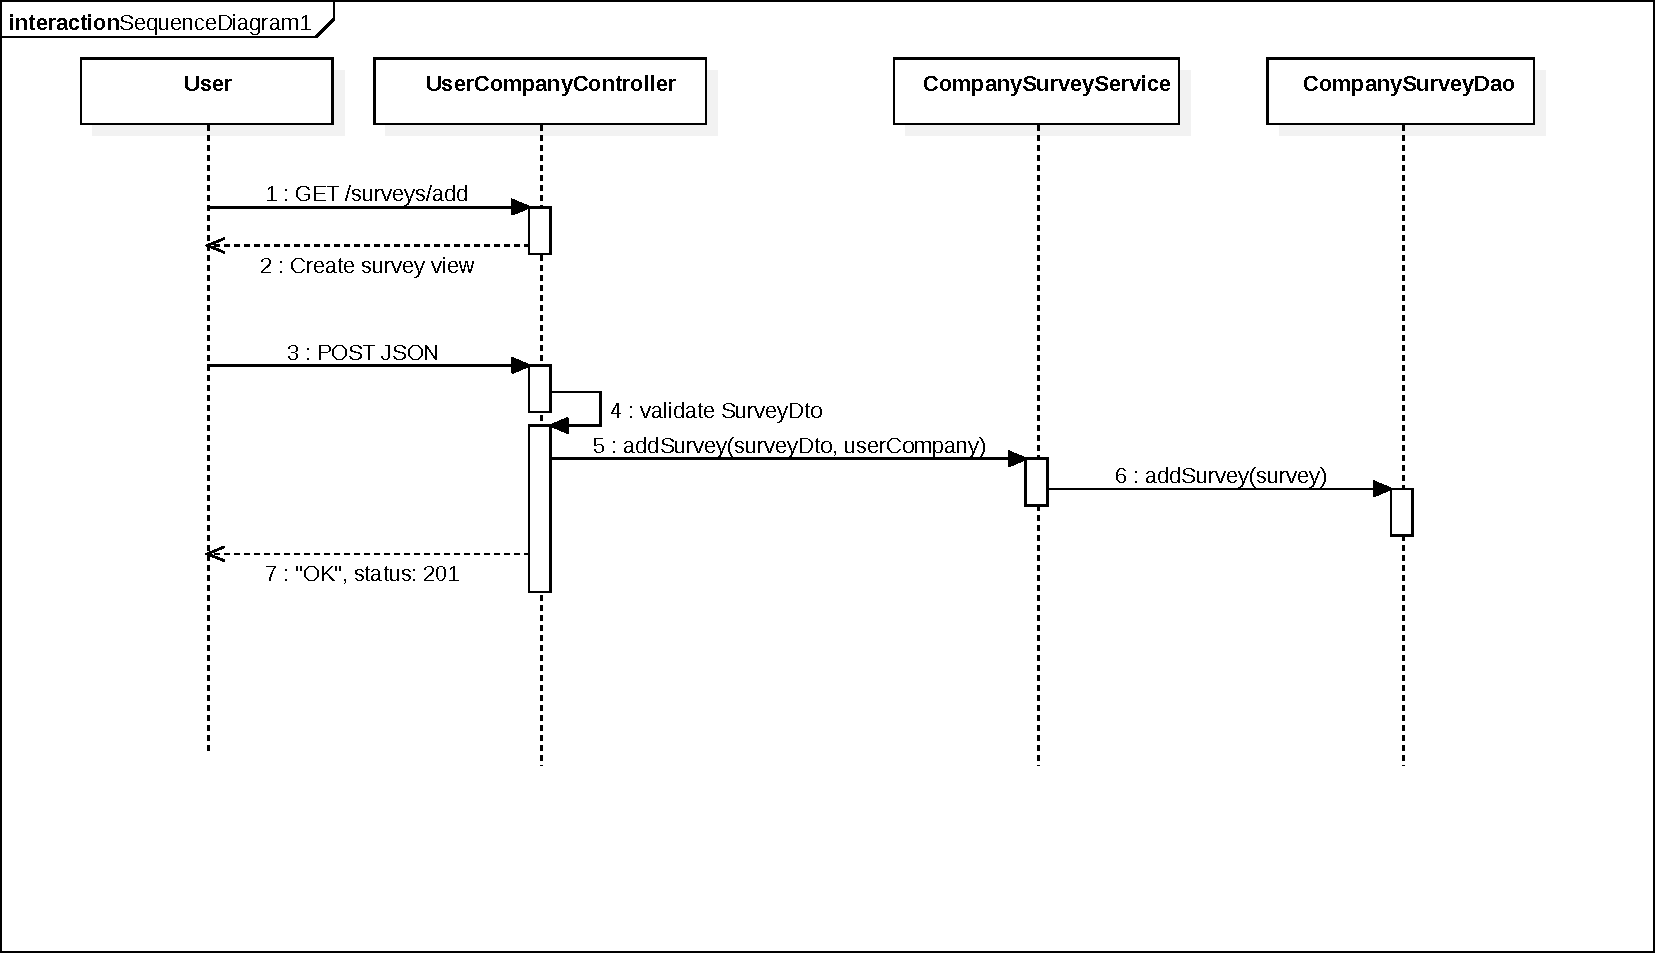
\includegraphics[width=15cm,height=20cm,keepaspectratio]{createSurveyPdf}
\caption{Diagram sekwencji dla poprawnego dodania nowej ankiety.}
\end{figure}

\paragraph{}
Na powyższym diagramie widoczne są połączenia między komponentami systemu dla dodawania nowej ankiety. Klasa \texttt{UserCompanyController} służy do komunikacji między użytkownikiem a resztą systemu. Walidacja zaznaczona na diagramie jako odwołanie \texttt{UserCompanyController} jest w rzeczywistości oddelegowana do walidatora, który dzięki zastosowanym w kodzie adnotacjom zna reguły walidacji pól w klasach. Oddelegowanie walidacji do walidatora jest oznaczone przy życiu adnotacji \texttt{@Validated} w argumencie kontrolera, który jest wiązany z ciałem żądania HTTP.

\section{Dodawanie kuponu}
\paragraph{}
Proces dodawania kuponu zaczyna się w momencie wysłania żądania GET przez zalogowaną firmę pod adres \texttt{/surveys/{id}/addVoucher}, gdzie {id} jest id wcześniej utworzonej ankiety. Po stronie klienta jest wczytywany panel do dodawania kuponu do wybranej ankiety. Panel pozwala na ustawienie rodzaju zniżki, jej wartości, opisu kuponu, a także czasu ważności kuponu.

\paragraph{}
Przy dodawaniu nowego kuponu tworzymy dane przypisywane do danego żądania i umieszczamy je jako atrybuty w \texttt{Modelu}. Dane te po wysłaniu odpowiedzi lub kolejnego żądania są wiązane z odpowiednimi obiektami w \texttt{Javie}. Dzięki takiemu rozwiązaniu można łatwo kontrolować walidację formularzy i łatwo sczytywać z nich dane, które następnie są procesowane w systemie.

\begin{center}
\begin{lstlisting}[caption={Listing kodu wywoływanego przy otrzymaniu żądania GET dla dodawania kuponu.},captionpos=b]
@RequestMapping(value = "/surveys/{id}/addVoucher", method = RequestMethod.GET)
    public String voucher(@AuthenticationPrincipal UserCompany userCompany, @PathVariable("id") int surveyId, Model model) {
        if(!checkForSurveyExistence(surveyId,userCompany)){
            return "error.html";
        }
        model.addAttribute("surveyId", surveyId);
        model.addAttribute("discountType", DiscountType.values());
        model.addAttribute("voucherForm",new VoucherForm());

        return "my_account/vouchers/add_voucher";
    }
\end{lstlisting}
\end{center}

W linijce pierwszej został określony mapping żądania \texttt{GET}. W linijkach 6-8 dodawane są atrybuty do modelu, które następnie będą zapełniane danymi, które dostarczy klient. W linijce 10 jako odpowiedź na żądanie jest zwracany HTML z widokiem panelu dodawania kuponu.

\paragraph{}
Po naciśnięciu przycisku \texttt{Zatwierdź}, do serwera wysyłane jest żądanie POST z obiektem \texttt{VoucherForm}. Obiekt klasy \texttt{VoucherForm} jest walidowany pod kątem zawartości niedozwolonych znaków oraz braku pól pustych. Jeżeli walidacja się powiedzie, do klienta zwracane są odpowiedzi analogicznie jak w przypadku procesu tworzenia ankiety.

\paragraph{}
Po udanej walidacji obiektu klasy \texttt{VoucherForm} wywoływana jest metoda \texttt{addVouchersForm} z serwisu \texttt{CompanySurveyService}, która dodaje utworzony kupon do bazy danych, łącząc go z odpowiednią ankietą. Zmapowany obiekt klasy \texttt{Voucher} jest w kolejnym kroku zapisywany w bazie danych, przy użyciu frameworka Hibernate. Proces dodawania kuponu jest zatem analogiczny, jak proces dodawania nowej ankiety.



\section{Wypełnianie ankiety}
\paragraph{}
Proces wypełniania ankiety zaczyna się od kliknięcia przez użytkownika przycisku \texttt{Wypełnij ankietę} na pasku nawigacyjnym. Użytkownik wybiera interesującą go firmę, a następnie ankietę. Ankiety są przedstawione w sposób jasno informujący o nagrodzie obowiązującej w zamian za jej wypełnienie. Wybranie ankiety blokuje jeden z kodów promocyjnych dla danego kuponu i wiąże go z identyfikatorem sesji użytkownika. Blokada kuponu dla użytkownika trwa przez 20 minut, a po upłynięciu tego czasu sesja wygaśnie i ankieta będzie musiała być wypełniona kolejny raz. 

\clearpage
\begin{center}
\begin{lstlisting}[caption={Listing kodu zwalniającego kod kuponu po wygaśnięciu sesji},captionpos=b]
@Override
    public void doFilter(ServletRequest request, ServletResponse response, FilterChain chain) throws IOException, ServletException {
        HttpServletRequest httpServletRequest = (HttpServletRequest) request;
        HttpSession session = httpServletRequest.getSession(true);
        Integer vDateId = (Integer) session.getAttribute("vCode");
        if (vDateId != null) {
            try {
                VoucherCodeDate voucherCodeDate = companySurveyService.getVoucherCodeDateById(vDateId);
                LocalDateTime localDateTime = LocalDateTime.now().minusMinutes(20);
                if (Date.from(localDateTime.atZone(ZoneId.systemDefault()).toInstant()).compareTo(voucherCodeDate.getUseDate()) > 0) {
                    session.removeAttribute("vCode");
                    companySurveyService.deleteVoucherCodeDate(vDateId);
                }
            } catch (Exception e) {
                if(!(e instanceof NullPointerException))
                    e.printStackTrace();
                session.removeAttribute("vCode");
            }
        }
        chain.doFilter(request, response);
    }
\end{lstlisting}
\end{center}

Powyższy listing prezentuje metodę z klasy \texttt{VoucherCodeFilter}. Filtr ten dodany jest do łańcucha filtrów, który jest rekurencyjnie przechodzony za każdym razem, gdy do serwera trafia żądanie. Po przejściu przez filtry otrzymujemy zmodyfikowane żądanie, które następnie jest procesowane przez \texttt{dispatcherServlet}, ustalający co to za żądanie i do jakiego adresu się odnosi. Filtry i \texttt{dispatcherServlet} są częścią frameworka \texttt{Spring Boot}. Po trafieniu żądania do filtra \texttt{VoucherCodeFilter} następuje sprawdzenie, czy w atrybutach sesji powiązanej z danym żądaniem znajduje się zablokowany kod kuponu. Jeżeli z identyfikatorem sesji związany jest jakiś kupon to w linijkach 8-10 sprawdzane jest czy nie minął czas przeznaczony na wypełnienie ankiety. Jeżeli czas został przekroczony to w linijkach 11-12 usuwane jest powiązanie sesji z kodem kuponu i kod wraca do puli.

\paragraph{}
Za proces wypełnienia ankiety i dostarczenia użytkownikowi kuponu odpowiada \texttt{Spring WebFlow}. W rozdziale trzecim zostało opisane działanie tego komponentu frameworku \texttt{Spring}. Służy on do tworzenia wieloetapowych formularzy, tzw. \textit{wizardów}. Dzięki zastosowaniu etapowego podejścia nie jest możliwe odwołanie się do adresu, który przekazuje kupon użytkownikowi, bez wcześniejszego wypełnienia ankiety. \texttt{WebFlow} umożliwia również kontrolę odblokowywania kuponów w przypadku, gdy użytkownik zrezygnuje z wysyłania ankiety. Po kliknięciu przycisku \texttt{Anuluj} w ankiecie wysyłane jest żądanie do serwera, które usuwa powiązanie kuponu z identyfikatorem sesji użytkownika. Gdy użytkownik zamknie okno przeglądarki kupon zostanie zwolniony dopiero po wygaśnięciu sesji.

\paragraph{}
Po każdym kroku formularza wypełniania ankiety, dane są walidowane. Nie jest możliwe przejście do kolejnego kroku, bez pozytywnej walidacji danych z poprzedniego etapu formularza. Do walidacji wypełnionej ankiety używana jest metoda \texttt{validate\-Answered\-Survey\-Form} z serwisu \texttt{Company\-Survey\-Service}.

\paragraph{}
Drugim krokiem formularza wieloetapowego jest podanie przez użytkownika danych statystycznych, takich jak wiek oraz kraj pochodzenia. Dane te również są walidowane. W tym kroku możliwe jest również podanie adresu e-mail, na który zostanie przesłany kupon. Jest to jednak pole opcjonalne, gdyż jednym z założeń niefunkcjonalnych aplikacji było zapewnienie użytkownikom anonimowości. W przypadku podania przez użytkownika adresu e-mail, wywoływana jest metoda \texttt{sendVoucherCodeEmail} z serwisu \texttt{mailService}, która przesyła kod na podany adres e-mail.

\begin{center}
\begin{lstlisting}[caption={Listing kodu wysyłającego e-mail.},captionpos=b]
private boolean send(String destinationEmail, String subject, Context ctx, 
				String eMailTemplate) {
        MimeMessage eMailMessage = mailSender.createMimeMessage();
        MimeMessageHelper eMailMessageHelper;
        try {
            eMailMessageHelper = new MimeMessageHelper(eMailMessage, true);
            eMailMessageHelper.setTo(destinationEmail);
            eMailMessageHelper.setSubject(subject);

            final String htmlContent = this.htmlTemplateEngine.
            					process(eMailTemplate, ctx);
            eMailMessageHelper.setText(htmlContent, true);
            mailSender.send(eMailMessage);
            return true;
        } catch (MessagingException e) {
            e.printStackTrace();
            return false;
        }
    }
\end{lstlisting}
\end{center}


Do wysyłania wiadomości e-mail przez system służy klasa \texttt{JavaMailSender}, która do komunikacji wykorzystuje protokół SMTP. Wszystkie wiadomości tworzone przez system, nie tylko te zawierające w sobie kupony promocyjne, są budowane w standardzie MIME. Framework \texttt{Spring} pozwala na łatwe tworzenie szablonów wiadomości e-mail, które można dynamicznie zapełniać zawartością w trakcie działania systemu. W powyższym listingu została przedstawiona metoda odpowiadająca za wysyłanie wiadomości e-mail w serwisie \texttt{MailService}. Na początku tworzony jest obiekt wiadomości w standardzie MIME, który jest następnie wypełniany wartościami takimi, jak adresat i nadawca. Zawartość wiadomości jest generowany przy użyciu silnika do szablonów pochodzącego z frameworka \texttt{Spring}. Przekazując do silnika szablonów kontekst wiadomości, zawierający niezbędne wartości, wykorzystywane przy dynamicznym tworzeniu treści maila, można w łatwy sposób uzyskać kod HTML, który następnie zostanie przesłany jako wiadomość do nadawcy.

\paragraph{}
Bezpośrednio przed wysłaniem do użytkownika kuponu wiadomością e-mail, bądź przed przekierowaniem użytkownika na stronę z kodem promocyjnym, następuje dodanie ankiety do bazy danych i usunięcie powiązania kuponu z identyfikatorem sesji. Dodanie wypełnionej ankiety do bazy danych jest przeprowadzane analogicznie, jak dodawanie kuponu lub ankiety. Obiekt jest zapisywany w bazie danych przy użyciu frameworka \texttt{Hibernate}, który zapewnia mapowanie relacyjno-obiektowe. Za usunięcie powiązania kuponu z identyfikatorem sesji odpowiada metoda \texttt{confirmAnsweringSurvey} z serwisu \texttt{CompanySurveyService}.
\clearpage

\begin{center}
\begin{lstlisting}[caption={Listing kodu blokującego kod promocyjny.},captionpos=b]
	@CacheEvict(value = {"surveyStat","ansList"},key = "#surveyId")
    @Override
    public VoucherCodeDto confirmAnsweringSurvey(Integer surveyId, 
    	AnsweredSurveyForm answeredSurveyForm, RequestContext requestContext) {
        HttpSession httpSession = ((HttpServletRequest) requestContext.getExternalContext().getNativeRequest()).getSession(true);
        Integer vCodeId = (Integer) httpSession.getAttribute("vCode");
        httpSession.removeAttribute("vCode");
        VoucherCode voucherCode = deployVoucherCode(vCodeId);
        String email = answeredSurveyForm.getEmail();
        if(email != null && !email.equals("")) {
            mailService.sendVoucherCodeEmail(voucherCode, email);
        }
        return new VoucherCodeDto(voucherCode);
    }
\end{lstlisting}
\end{center}

Powyższy listing pokazuje działanie metody odpowiedzialnej za dostarczenie kuponu do użytkownika i zwolnienie jego powiązania z identyfikatorem sesji. W linijkach 5-8 usuwane jest powiązanie kodu kuponu z identyfikatorem sesji, natomiast w linijkach 9-12 jest wysyłana wiadomość e-mail, o ile użytkownik podał opcjonalny adres e-mail. Metoda zwraca \texttt{Data Transfer Object} \texttt{VoucherCodeDto}, który następnie jest wyświetlany użytkownikowi po przekierowaniu. Warto również zwrócić uwagę na dezaktualizację cache'a po dodaniu nowej ankiety. Cache jest używany w systemie do przechowywania statystyk. Więcej o cache'u oraz statstykach można przeczytać w podrozdziale 4.6.

\begin{figure}[h]
\centering
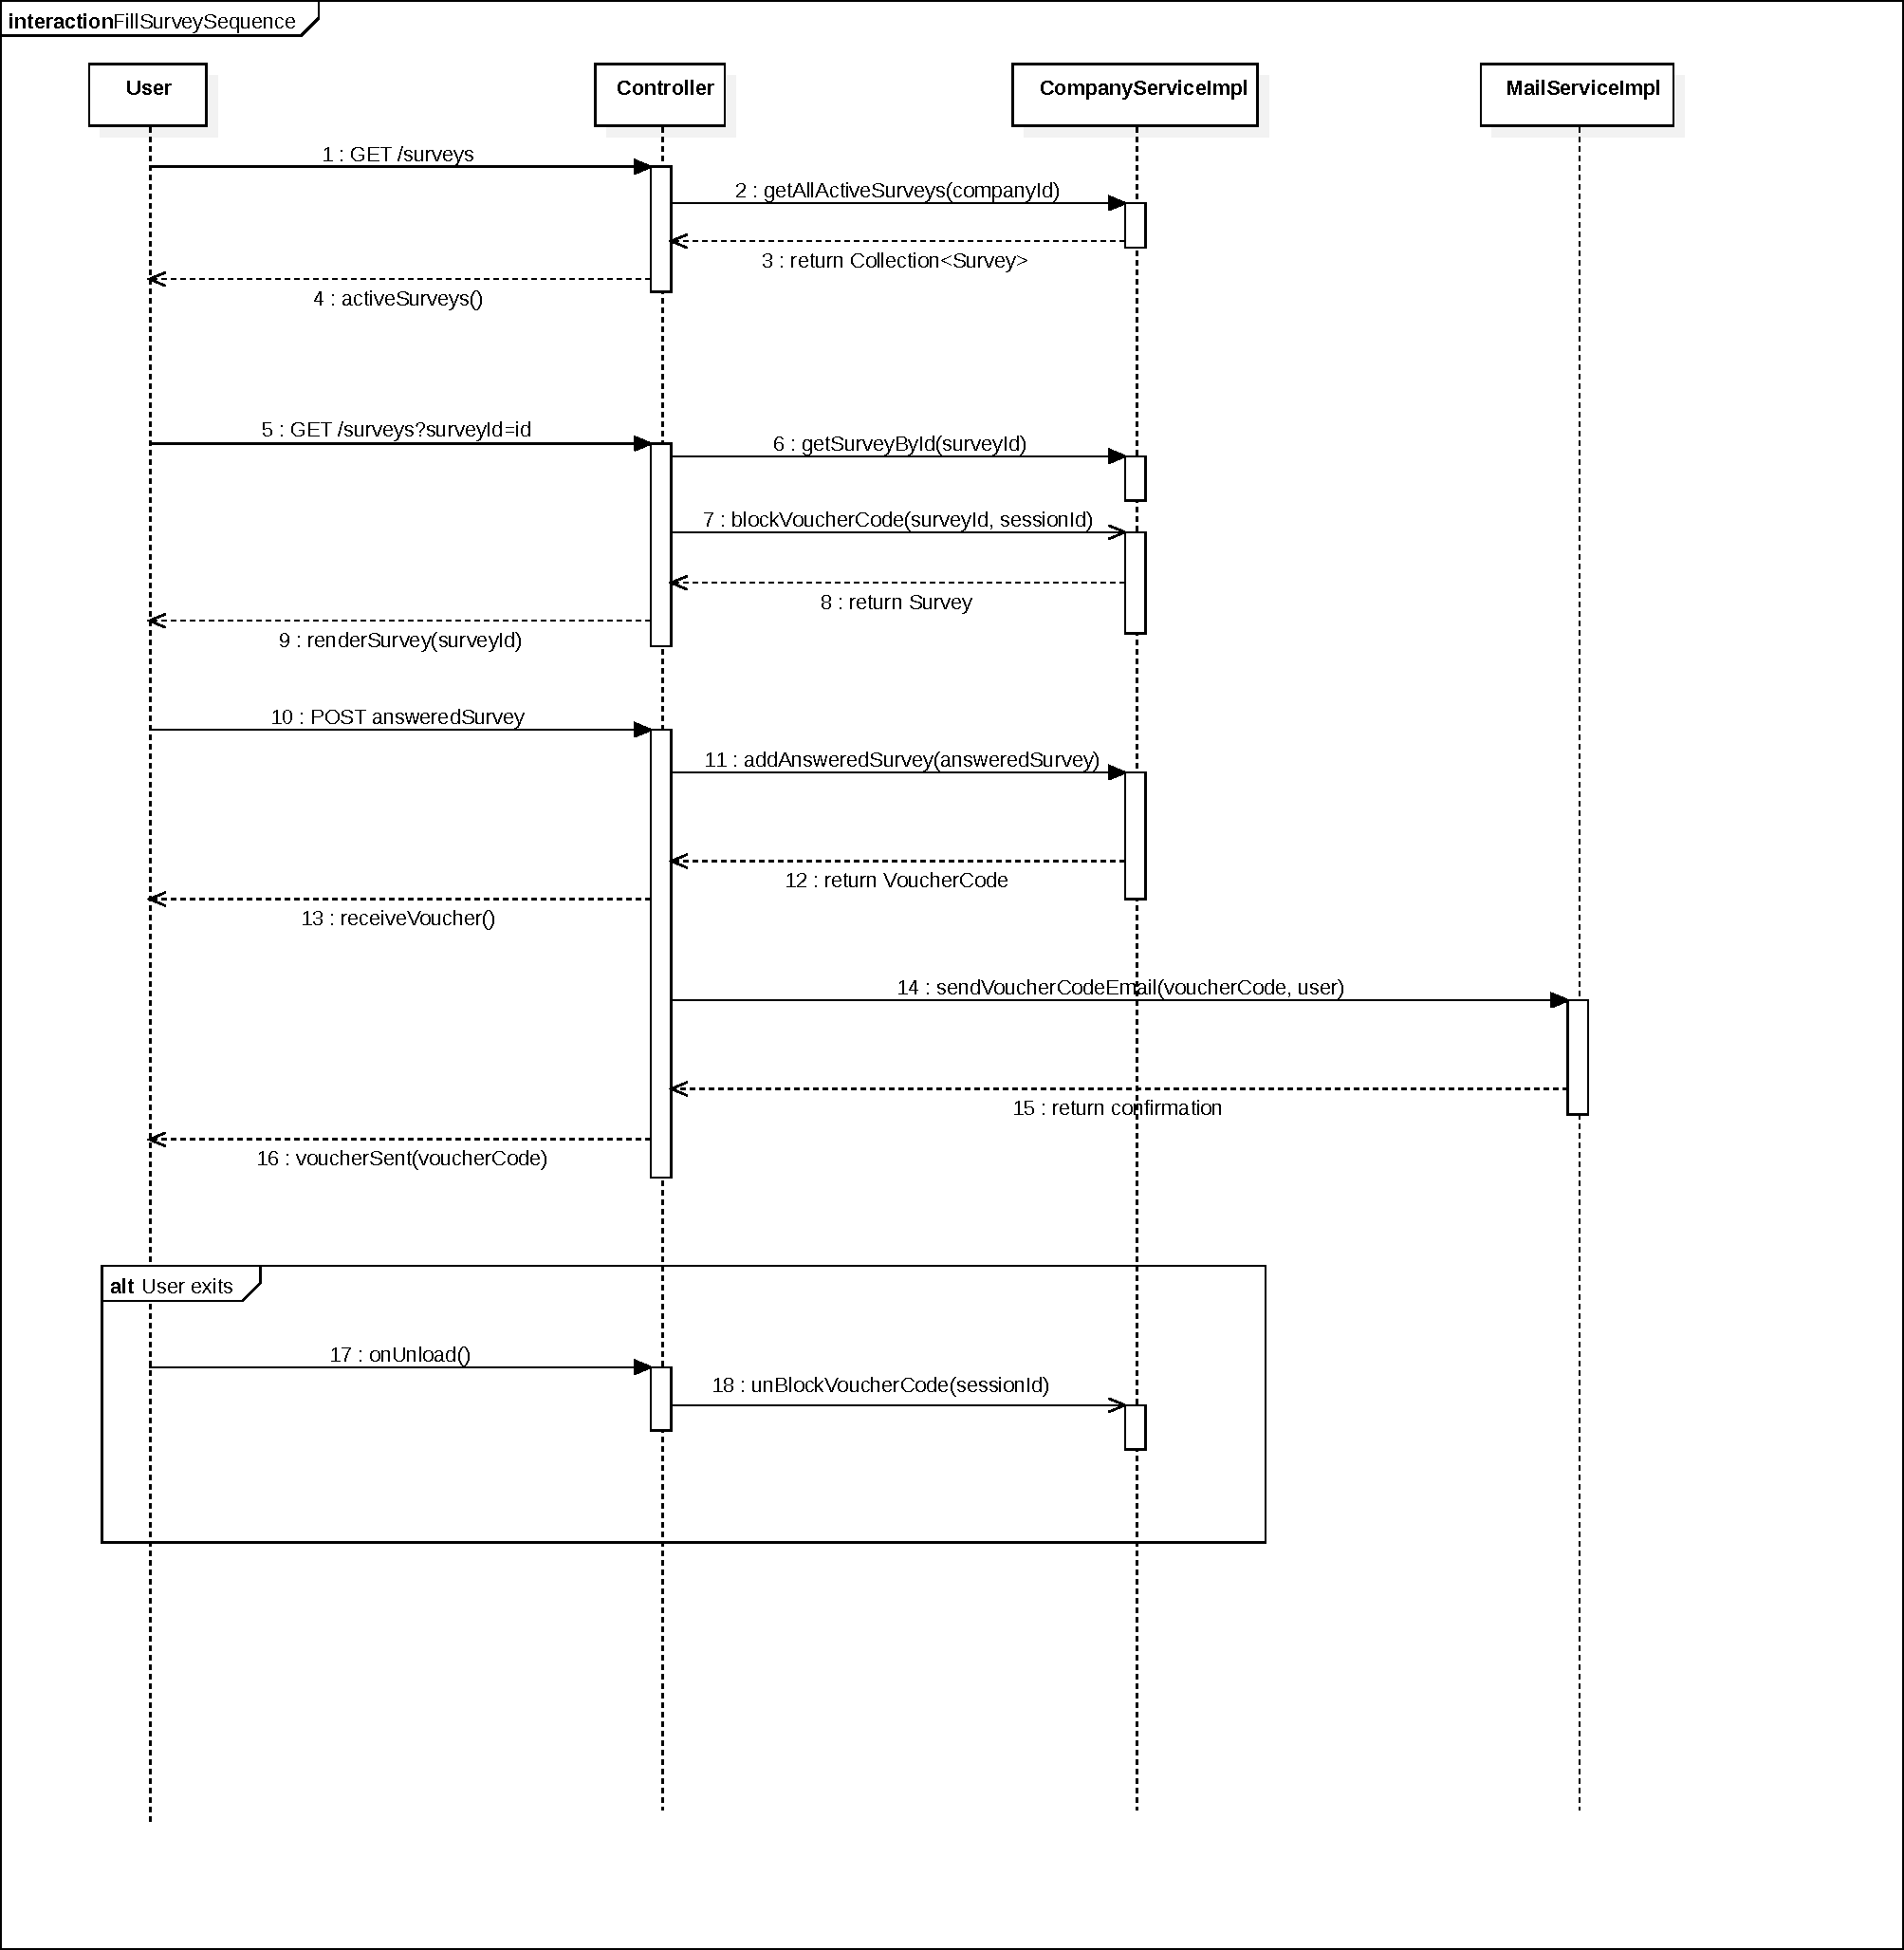
\includegraphics[width=10cm,height=10cm,keepaspectratio]{SequenceUMLFillSurvey}
\caption{Diagram sekwencji dla wypełniania ankiety.}
\end{figure}

Powyższy diagram sekwencji przedstawia proces wypełniania ankiety w aplikacji webowej. 

\section{Wypełnianie ankiety przez aplikację mobilną}
\paragraph{}
Aby móc wypełnić ankietę w aplikacji mobilnej, w tle wykonuje się wiele procesów zarówno aby dostarczyć odpowiednią ankietę do aplikacji mobilnej, jak i odpowiedzi udzielone przez użytkownika do serwera. Najpierw aplikacja mobilna, po wybraniu przez użytkownika firmy oraz ankiety, przesyła za pomocą frameworka retrofit2 metodą post informacje na temat interesującej użytkownika ankiety.
Serwer w momencie kiedy odbierze informacje, tworzy sesje dla naszej aplikacji, rezerwuje jeden kupon dla danego tokena sesji, oraz przesyła jako odpowiedź wyżej wymieniony token, wraz z pytaniami i typami pytań do konkretnie wybranej przez nas ankiety. Aplikacja mobilna odbierając plik JSON, zapisuje sobie plik cookie (który zapewnia nam utrzymanie sesji), oraz załącza pytania do listview w naszej nowo utworzonej aktywności. W trakcie dołączania pytań, aplikacja weryfikuje dla każdego z pytań jakiego jest ono rodzaju, i na tej podstawie tworzy kolejne elementy listview aby wyglądem pasowały do typu pytania. Na samym dole jest tworzony przycisk, służący do zaakceptowania naszej ankiety. Aplikacja w momencie gdy ankieta jest gotowa do wypełniania, umożliwia wysłanie ankiety dopiero wtedy, gdy zweryfikuje że odpowiedzi do ankiet są „niepuste”. 
Gdy użytkownik naciśnie przycisk akceptujący ankietę, i aplikacja dokona poprawnej walidacji ankiety następuje pobranie odpowiedzi z poszczególnych pól ankiety, umieszczenie ich w pliku JSON, oraz przesłanie ich metodą POST do serwera. Do naszej metody załączany jest plik cookies w którym przechowywany jest token sesji. W następnym kroku serwer przetwarza informacje przekazane przez aplikacje, zaś aplikacja czeka na odpowiedź z serwera. Jeżeli serwer nie był w stanie przetworzyć danych, (albo akurat w momencie gdy wysyłaliśmy nasza ankietę nie było zasięgu) nasza aplikacja mobilna informuje użytkownika o wystąpieniu błędu i cofa nas do ankiety. W przeciwnym przypadku serwer powinien zwrócić do aplikacji mobilnej plik JSON wraz z kodem promocyjnym oraz pozostałymi informacjami odnośnie otrzymanego vouchera. Gdy aplikacja odbierze wyżej wymieniony kod promocyjny, z automatu przekieruje nas do zakładki z posiadanymi kuponami.
W aplikacji mobilnej w zależności od tego czy podamy adres e-mail, możemy otrzymać kupon dodatkowo na konto e-mail. Warto dodatkowo zwrócić uwagę na fakt, że aplikacja została zaopatrzona w obsługę rezygnacji z wypełniania ankiety. Oznacza to, że w momencie gdy będziemy chcieli w aplikacji wrócić do menu głównego, albo zakończymy działanie aplikacji, to nasz program za pomocą metody POST wyśle informacje do serwera wraz z tokenem sesji o odblokowaniu vouchera który był dla nas wcześniej zarezerwowany.

\section{Statystyki}
\paragraph{}
\begin{lstlisting}[caption={Listing kodu pobierającego statystyki dla danej ankiety.},captionpos=b] 
@Cacheable("surveyStat")
@Override
public SurveyStatisticsDto getSurveysStatistics(int surveyId) {
	Collection<AnsweredSurvey> answeredSurveys = getAllAnsweredSurveysWithDetails(surveyId);
	Survey survey = companySurveyService.getSurveyByIdWithQuestion(surveyId);
	SurveyStatisticsDto surveyStatisticsDto = new SurveyStatisticsDto();
	surveyStatisticsDto.setAmmount(answeredSurveys.size());
	surveyStatisticsDto.setSurveyName(survey.getSurveyName());

	//average age
	double averageAge = answeredSurveys.stream().mapToInt(a -> a.getUser().getAge()).average().orElse(0.0);
	surveyStatisticsDto.setAge(averageAge);

	//average country
	List<String> countries = answeredSurveys.stream().map(a -> a.getUser().getCountry()).collect(Collectors.groupingBy(Function.identity(), Collectors.counting())).entrySet().stream().sorted(Comparator.comparingLong(Map.Entry::getValue)).limit(3).map(Map.Entry::getKey).collect(Collectors.toList());
	while (countries.size() != 3)
		countries.add("N/A");
	surveyStatisticsDto.setCountry(countries.toArray(new String[3]));
	
	if (answeredSurveys.size() == 0)
		return surveyStatisticsDto;

	//initialaizing iterators
	Iterator<AnsweredSurvey> answeredSurveyIterator = answeredSurveys.iterator();
	Iterator<Question> qIterator = survey.getQuestions().iterator();
	Iterator<Answer>[] aIteratorArray = new Iterator[answeredSurveys.size()];
	IntStream.range(0, aIteratorArray.length).forEach(i -> aIteratorArray[i] = answeredSurveyIterator.next().getAnswersList().iterator());

	int answersSize = answeredSurveys.size();
	List<QuestionStatisticsDto> questionStatisticsDtoList = surveyStatisticsDto.getQuestionWithAnswersList();
	while (qIterator.hasNext()) {
		Question q = qIterator.next();
		QuestionType qType = q.getQuestionType();
		QuestionStatisticsDto questionStatisticsDto = new QuestionStatisticsDto();
		questionStatisticsDto.setQuestionBody(q.getQuestionBody());
		questionStatisticsDto.setQuestionType(qType);

		switch (qType) {
			case OPEN:
				Arrays.stream(aIteratorArray).forEach(Iterator::next);
				questionStatisticsDto.setAnswers(null);
				break;
			case RANGED:
				double average = 0;
				for (Iterator<Answer> anAIteratorArray : aIteratorArray) {
					String temp = anAIteratorArray.next().getAnswer();
					average += Double.parseDouble(temp);
				}
				questionStatisticsDto.getAnswers()[0].setAnswersStat(Double.toString(average / answersSize));
				break;
			default:
				double[] apperances = new double[4];
				for (Iterator<Answer> anAIteratorArray : aIteratorArray) {
					Answer a = anAIteratorArray.next();
					String[] splited = a.getAnswer().split(",");
					for (String s : splited) {
						switch (s) {
							case "A":
								apperances[0]++;
								break;
							case "B":
								apperances[1]++;
								break;
							case "C":
								apperances[2]++;
								break;
							case "D":
								apperances[3]++;
		           		}
					}
				}
				IntStream.range(0, apperances.length).forEach(a -> questionStatisticsDto.getAnswers()[a].setAnswersStat(Double.toString(100 * apperances[a] / answersSize)));
				questionStatisticsDto.setPossibleAnswers(q.getPossibleAnswers());
				break;
		}
            
		questionStatisticsDtoList.add(questionStatisticsDto);
	}
	return surveyStatisticsDto;
}
\end{lstlisting}
Na powyższym listingu warto zauwazyć, że metoda jest cache'owana tj. zapmietywane jest przez serwer wartość, która zostanie zwrócona dla danego argumentu. Przy dużej liczbie rozwiązanych ankiet obliczanie statystyk, może być stosunkow czasochłonne, a sam cache zapewnia nam, że nie statystyki dla tych samych danych nie będa liczone kilkukrotnie.
\paragraph{}
Pierwszym etapem jest pobranie z bazy danych listy wypełnionych ankiet, a następnie policzenie średniego wieku przy użyciu \textbf{Stream API}, \textbf{Lamba Expressions} oraz klasy generycznej \textbf{Optional<T>}. Przy użyiu tych samych ``narzędzi'' dostępnych w Javie zostaje obliczona posortowana lista krajów, względem częstości wypełniania danej ankiety w tym kraju. Lista ta jest ograniczona do $3$ najlepszych wyników, a w przypadku gdy zawiera ona mniej niż $3$ kraje zostaje wypełniona wyrażeniem ``N/A''. W przypadku gdy ankieta nie została rozwiązana zwracany jest pusty obiad, w innej sytuacji w pętli iterujemy po pytaniach w kolejnych odpowiedziach, tzn. na początku dla każdej odpowiedzi na pytanie numer $1$ liczymy statystyki, następnie robimy to dla każdej istniejącej odpowiedzi na pytanie numer $2$ itd. Jeżeli pytanie jest pytaniem typu ``ranged'' (tj. w skali od 0 do 10) liczona jest średnia arytmetyczna wyniku. Jeżeli jest to pytanie typu zamkniętego lub zamkniętego wieloktronego wyboru przy pomocy \textbf{Stream API}, \textbf{Lamba Expressions} oraz klasy generycznej \textbf{Optional<T>} liczona jest częstość występowania danej odpowiedzi (która należy do zbioru $\{A,B,C,D\}$). Następnie przy pomocy set'erów i get'erów klasy \textbf{SurveyStatisticsDto} obliczone wcześniej dane zostają ``wrzucone'' do obiektu wyjściowego, który jest ostatecznie zwracany przez metode.
